
\subsection{Diseño de interfaz}
Al tratarse del primer incremento, fué de vital importancia comenzar a definir la guía de diseño de la interfaz de usuario. En primer lugar, se definió una paleta de colores \figref{fig:ui_palette} y su uso en distintos componentes de la interfaz \figref{fig:ui_guide}.

\begin{figure}[H]
    \centering
    \begin{subfigure}[t]{0.48\textwidth}
        \centering
        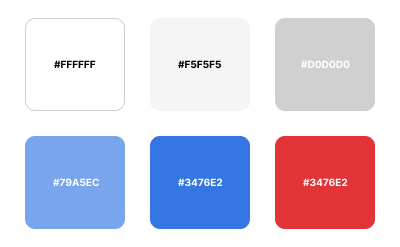
\includegraphics[width=1\textwidth]{Ilustraciones/desarrollo/incremento1/diseño/color_palette.jpg}
        \caption{Paleta de colores}\label{fig:ui_palette}
    \end{subfigure}
    \hfill
    \begin{subfigure}[t]{0.48\textwidth}
        \centering
        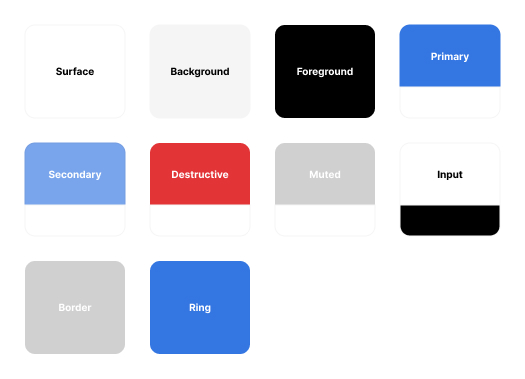
\includegraphics[width=\textwidth]{Ilustraciones/desarrollo/incremento1/diseño/color_scheme.jpg}
        \caption{Guía de colores. Los cuadros con dos colores definen arriba el fondo y abajo el color del texto o elementos en primer plano}\label{fig:ui_guide}
    \end{subfigure}\caption{Colores utilizados en la interfaz}\label{fig:ui_colors}
\end{figure}

En segundo lugar, se diseñó el isologo de la aplicación web \figref{fig:ui_logo}, el cual combina el timple con el nombre de la aplicación web \textbf{Timple Tabs}.

\begin{figure}[H]
    \centering
    
\includegraphics[width=0.5\textwidth]{Ilustraciones/desarrollo/incremento1/diseño/logo_2.png}
    \caption{Isologo de la aplicación web}\label{fig:ui_logo}
\end{figure}

En tercer lugar, se diseñaron algunos de los elementos comunes de la interfaz de usuario. Para este primer incremento fué fundamental el diseño de botones \figref{fig:ui_buttons}, campos de formulario \figref{fig:ui_fields}, dialogos \figref{fig:dialog}, información desplegable \figref{fig:dropdown_info}. Algunos de estos elementos hacen uso de iconos, por lo cual se decidió utilizar la biblioteca pública \textbf{Lucide Icons} \cite{lucide_icons}.

\begin{figure}[H]
    \centering
    \begin{subfigure}[t]{0.48\textwidth}
        \centering
        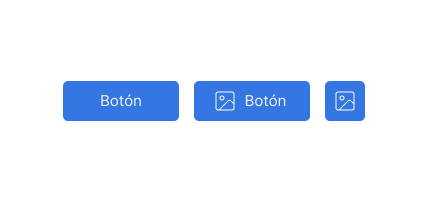
\includegraphics[width=1\textwidth]{Ilustraciones/desarrollo/incremento1/diseño/buttons.jpg}
        \caption{Botones y sus variantes según espacio}\label{fig:ui_buttons_variants}
    \end{subfigure}
    \hfill
    \begin{subfigure}[t]{0.48\textwidth}
        \centering
        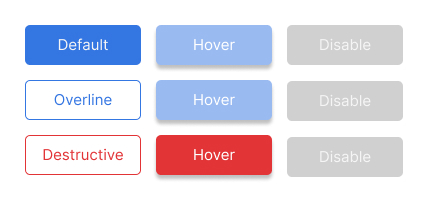
\includegraphics[width=1\textwidth]{Ilustraciones/desarrollo/incremento1/diseño/button_color_scheme.jpg}
        \caption{Botones y sus variantes según función y estado}\label{fig:ui_buttons_color}
    \end{subfigure}
    \vspace{1em}
    \begin{subfigure}[t]{\textwidth}{
        \centering
        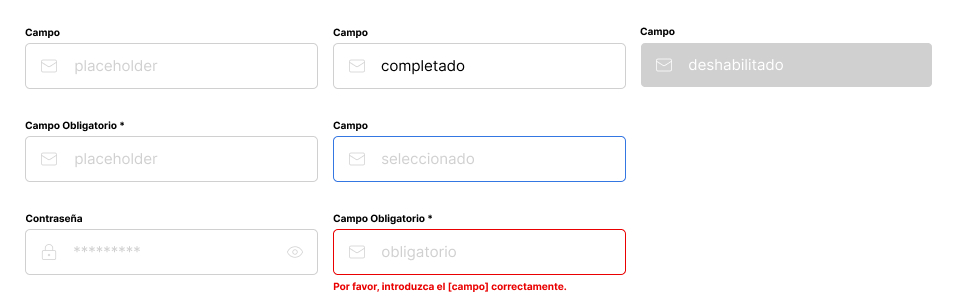
\includegraphics[width=\textwidth]{Ilustraciones/desarrollo/incremento1/diseño/fields.jpg}
        \caption{Campos y sus variantes según función y estado}\label{fig:ui_fields}}    
    \end{subfigure}
    \vspace{1em}
    \begin{subfigure}[t]{0.38\textwidth}
        \centering
        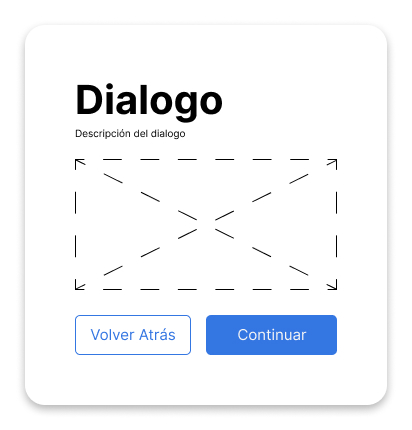
\includegraphics[width=1\textwidth]{Ilustraciones/desarrollo/incremento1/diseño/dialog.jpg}
        \caption{Dialogo sin contenido}\label{fig:dialog}
    \end{subfigure}
    \hfill
    \begin{subfigure}[t]{0.58\textwidth}
        \centering
        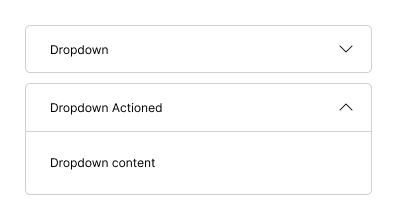
\includegraphics[width=1\textwidth]{Ilustraciones/desarrollo/incremento1/diseño/dropdown_info.jpg}
        \caption{Información desplegable}\label{fig:dropdown_info}
    \end{subfigure}
    
    \caption{Diseño de elementos comunes}\label{fig:ui_buttons}
\end{figure}

Utilizando los elementos anteriores se realizó el diseño de las pantallas correspondientes al inicio de sesión \figref{fig:ui_login}, recuperación de contraseña \figref{fig:passrec}, registro \figref{fig:ui_register_empty}, perfil \figref{fig:ui_profile} y ajustes de cuenta \figref{fig:ui_settings}. 

\begin{figure}[H]
    \centering
    \begin{subfigure}[t]{0.2\textwidth}
        \centering
        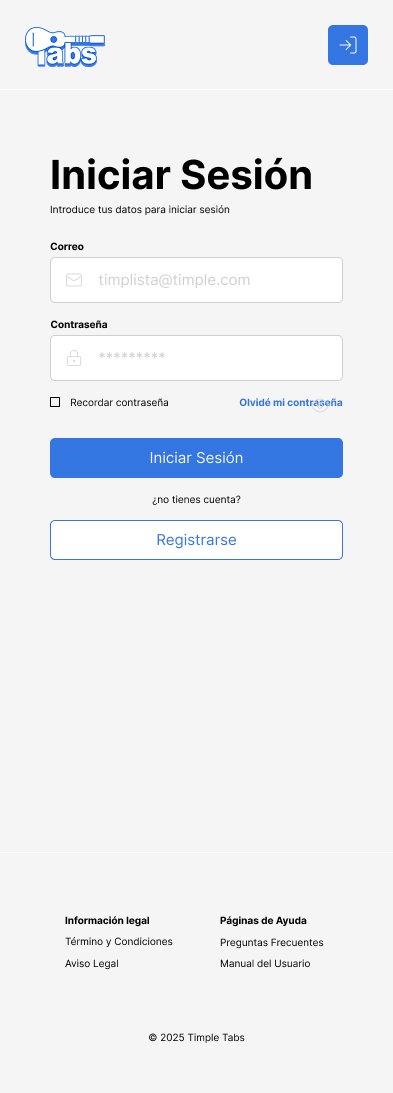
\includegraphics[width=1\textwidth]{Ilustraciones/desarrollo/incremento1/diseño/login.jpg}
        \caption{Diseño de página de inicio de sesión}\label{fig:ui_login}
    \end{subfigure}
    \hfill
    \begin{subfigure}[t]{0.2\textwidth}
        \centering
        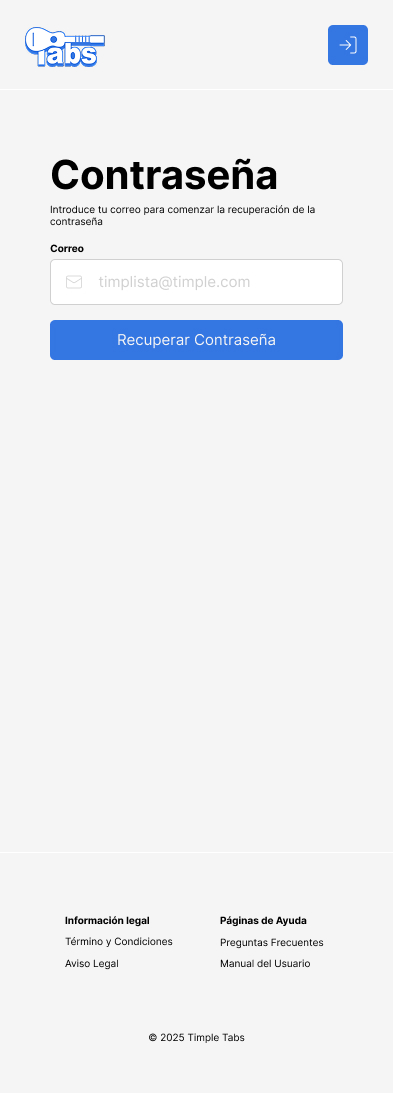
\includegraphics[width=1\textwidth]{Ilustraciones/desarrollo/incremento1/diseño/password_recovery.jpg}
        \caption{Diseño de página de recuperación de contraseña}\label{fig:passrec}
    \end{subfigure}
    \hfill
    \begin{subfigure}[t]{0.2\textwidth}
        \centering
        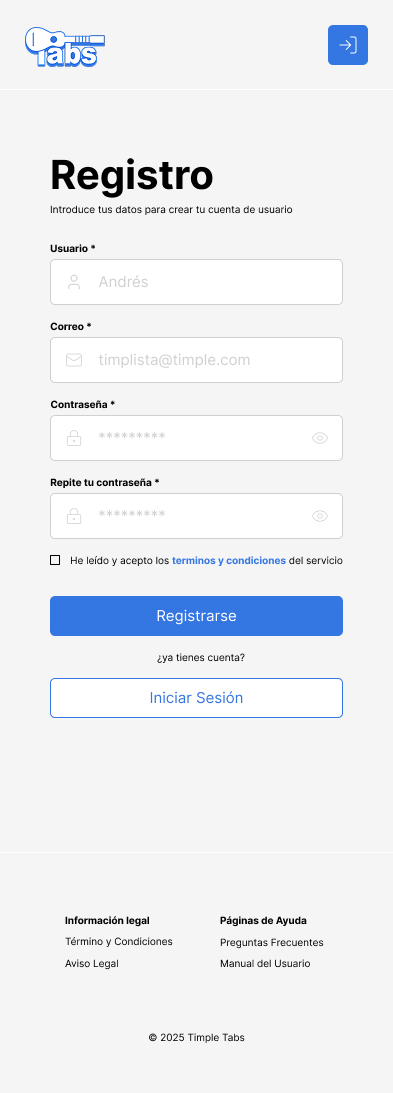
\includegraphics[width=1\textwidth]{Ilustraciones/desarrollo/incremento1/diseño/register.jpg}
        \caption{Diseño de pantalla de registro de usuario con campos vacios}\label{fig:ui_register_empty}
    \end{subfigure}
    \hfill
    \begin{subfigure}[t]{0.2\textwidth}
        \centering
        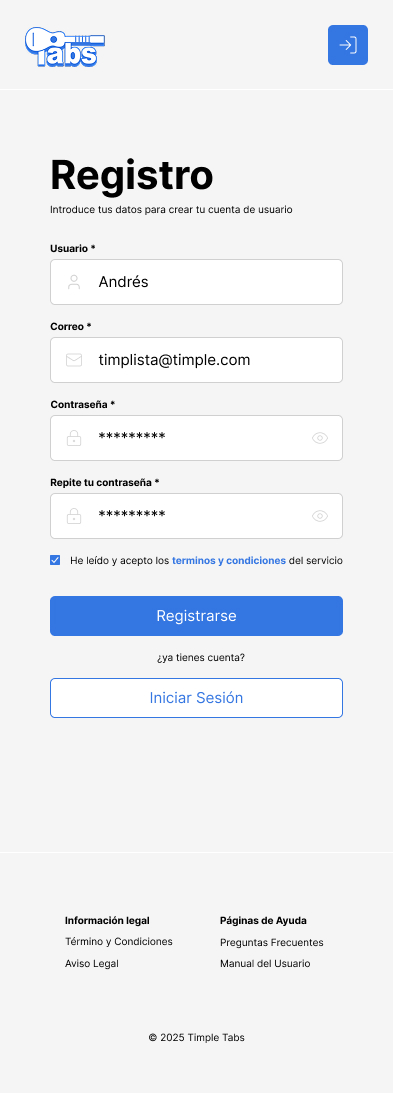
\includegraphics[width=1\textwidth]{Ilustraciones/desarrollo/incremento1/diseño/register_filled.jpg}
        \caption{Diseño de pantalla de registro de usuario con campos completados}\label{fig:ui_register_fill}
    \end{subfigure}
    \hfill
    \begin{subfigure}[t]{0.2\textwidth}
        \centering
        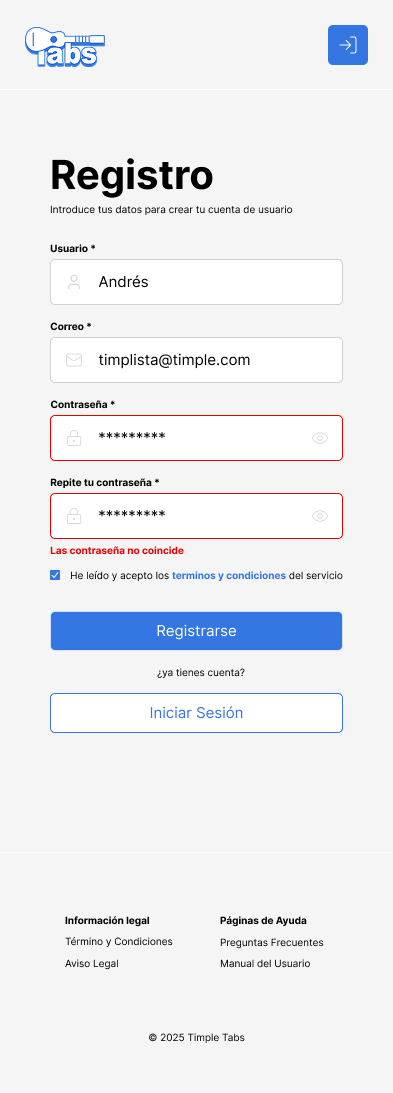
\includegraphics[width=1\textwidth]{Ilustraciones/desarrollo/incremento1/diseño/register_error.jpg}
        \caption{Diseño de pantalla de registro de usuario con campos incorrectos}\label{fig:ui_register_fail}
    \end{subfigure}
    \hfill
    \begin{subfigure}[t]{0.2\textwidth}
        \centering
        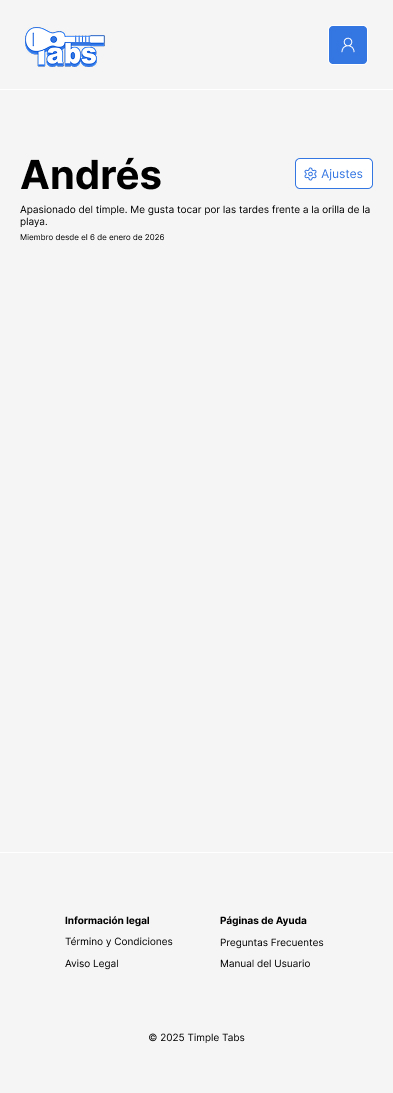
\includegraphics[width=1\textwidth]{Ilustraciones/desarrollo/incremento1/diseño/profile.jpg}
        \caption{Diseño de página de perfil de usuario}\label{fig:ui_profile}
    \end{subfigure}
    \hfill
    \begin{subfigure}[t]{0.2\textwidth}
        \centering
        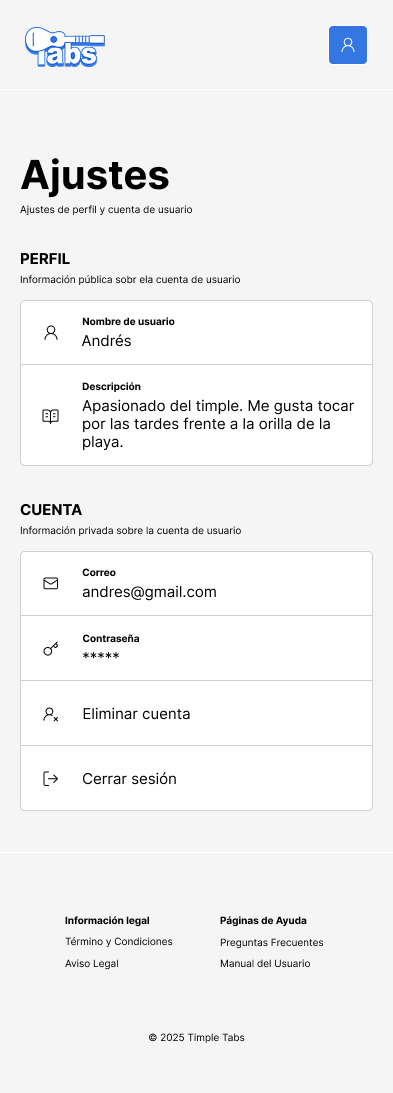
\includegraphics[width=1\textwidth]{Ilustraciones/desarrollo/incremento1/diseño/settings.jpg}
        \caption{Diseño de página de perfil de usuario}\label{fig:ui_settings}
    \end{subfigure}
    \vspace{1em}
    \caption{Diseño de página de ajustes de cuenta de usuario}\label{fig:ui_smt}
\end{figure}

Los anteriores han sido diseñados con el enfoque mobile-first, asegurando una correcta visualización y usabilidad en dispositivos móviles y adaptándose a pantallas de mayor tamaño mediante un diseño responsivo \figref{fig:ui_login_desktop}.

\begin{figure}[H]
    \centering
    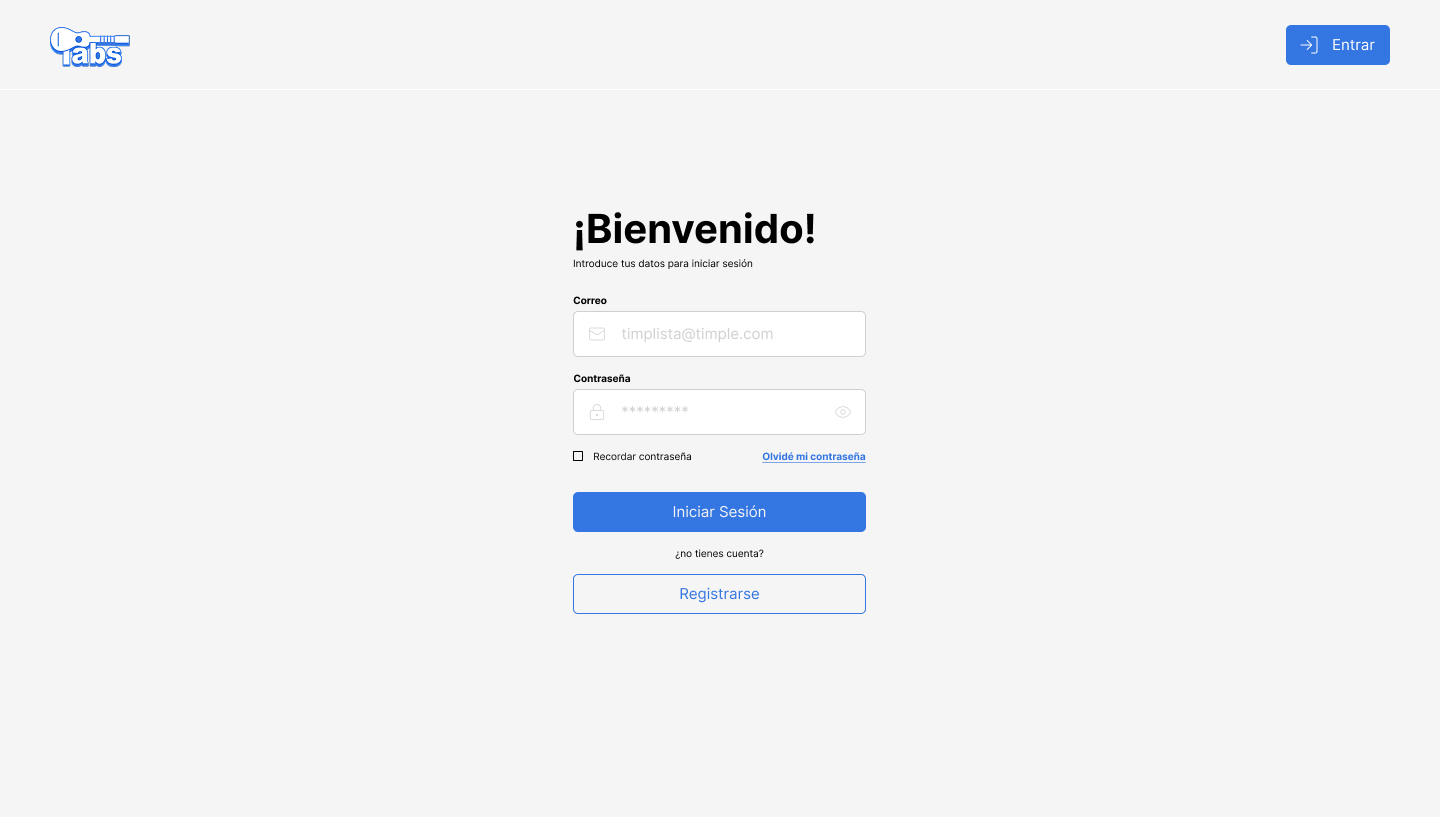
\includegraphics[width=0.8\textwidth]{Ilustraciones/desarrollo/incremento1/diseño/login_big.jpg}
    \caption{Diseño de página de inicio de sesión en pantallas grandes}\label{fig:ui_login_desktop}
\end{figure}